%!TEX root = ../username.tex


\chapter{Human Sensory Perception: Biological and Cognitive}\label{Perception}

 VR is created through an exchange of information between the user and the virtual environment. For VR to be realistic, there must be a certain degree of responsiveness to a user's actions or inputs. Interaction within a virtual environment can be broken down into three categories: manipulation, navigation, and communication. 
 Manipulation allows the user to interact and make modifications to the virtual world and the objects within it. This interaction increases mental presence within an environment by promoting creativity and expression. Navigation permits the user to maneuver through the world, giving an illusion of depth within an environment. Effective navigation techniques require the user to create a mental picture of the environment, inherently promoting mental presence. Communication enables interaction between users and intermediaries in a virtual environment. Having multiple users in an environment enables an exchange of information and experiences \cite{mihelj_apps}.

%\section{Human Interaction} \label{interaction}


%%%%%%%%%%%%%%%%%%%	
%				  %	
%      SIGHT      %
%				  %
%%%%%%%%%%%%%%%%%%%

\section{Human Visual System} \label{sight}


Visual perception is considered to be the most dominant sense. Human cognition is oriented around vision, demonstrated by the fact that the visual system is given precedence over the other senses when conflicting inputs are present \cite{gobbetti}. A large area of the brain is dedicated to interpreting how we process the information gained from visible light. Because human behavior is so visually oriented, visual perception is given the utmost priority during any virtual experience. Due to the significance of visual perception, the frequency at which intermittent stimulus appear to be steady and in constant motion, or the critical fusion frequency, is an integral aspect of the visual system. Light perception, color perception, depth perception, field-of-view, and critical fusion frequency are vital components of the visual system and are discussed briefly in the next subsections with an emphasis on depth perception. 

\subsection{Light Perception} \label{sight_perception} 

It is important to understand exactly how light perception works. Figure \ref{fig:humaneye} is useful for the following description. First, visible light from the environment enters the eye through the transparent cornea. The light intensity is controlled via the pupil, which can limit the amount of light entering the eye by dilating or contracting. Behind the pupil is the lens, whose job it is to focus light on the retina. The lens, which is attached and controlled by the ciliary muscle, is able to contract in order to change its thickness. Changing the thickness of the lens enables objects at different distances from the eye to be clearly seen \cite{mihelj_apps}. 
%\cite{VR Tech and Apps}.

\begin{figure}[h]
	\centering
	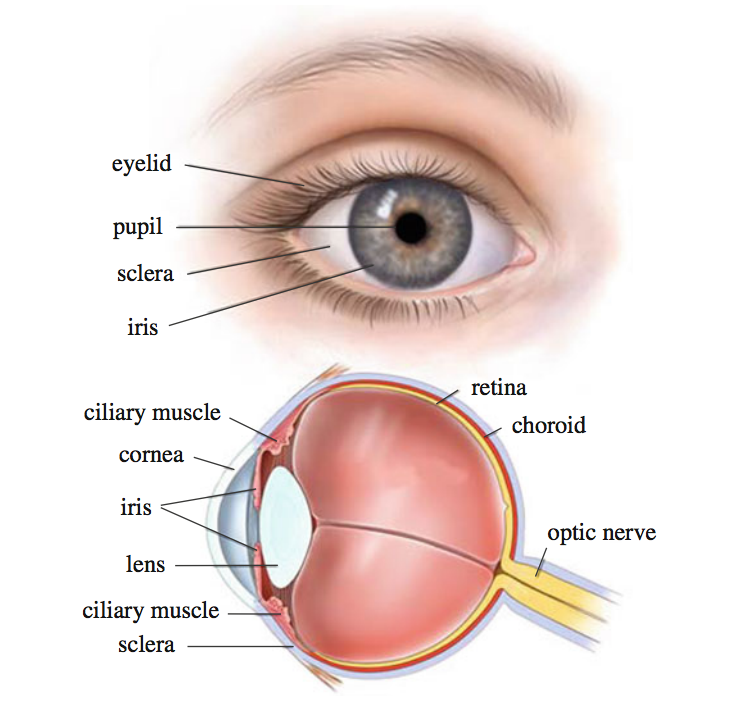
\includegraphics[width=.5\textwidth]{humanEye}
	%cite VR tech and Apps
	\caption{The human eye \cite{mihelj_apps}.}
	\label{fig:humaneye}
\end{figure}

\par The retina contains photoreceptors that are specialized light-sensing nerve endings. Photoreceptors can be divided into cones and rods. Cones sense colors, react quickly to light intensity changes, and are less sensitive to light. Rods do not sense color, are more sensitive to light, and allow sight during conditions with low levels of light. The light picked up by these receptors is then converted into an electrochemical signal that travels across the optic nerve. The optic nerve connects to the visual cortex in the brain, which turns the incoming signals into the images we then see \cite{mihelj_apps}.

\subsection{Color Perception} \label{color_perception} 

Using the cones in the retina, the human eye is able to sense varying levels of color. There are three types of cones in the eye that are able to pick up different wavelengths of light. The tiny wavelengths of visible light that humans can "see" range from 380 to 700 billionths of a meter, expressed as nanometers or nm. The first cone type senses red light (564-580nm), the second type senses green light (534-545nm), and the third type of cone picks up blue light (420-440nm) \cite{mihelj_apps}. The shorter wavelengths are known as ultraviolet light and the longer wavelengths are called infrared light.


\begin{figure}[h]
	\centering
	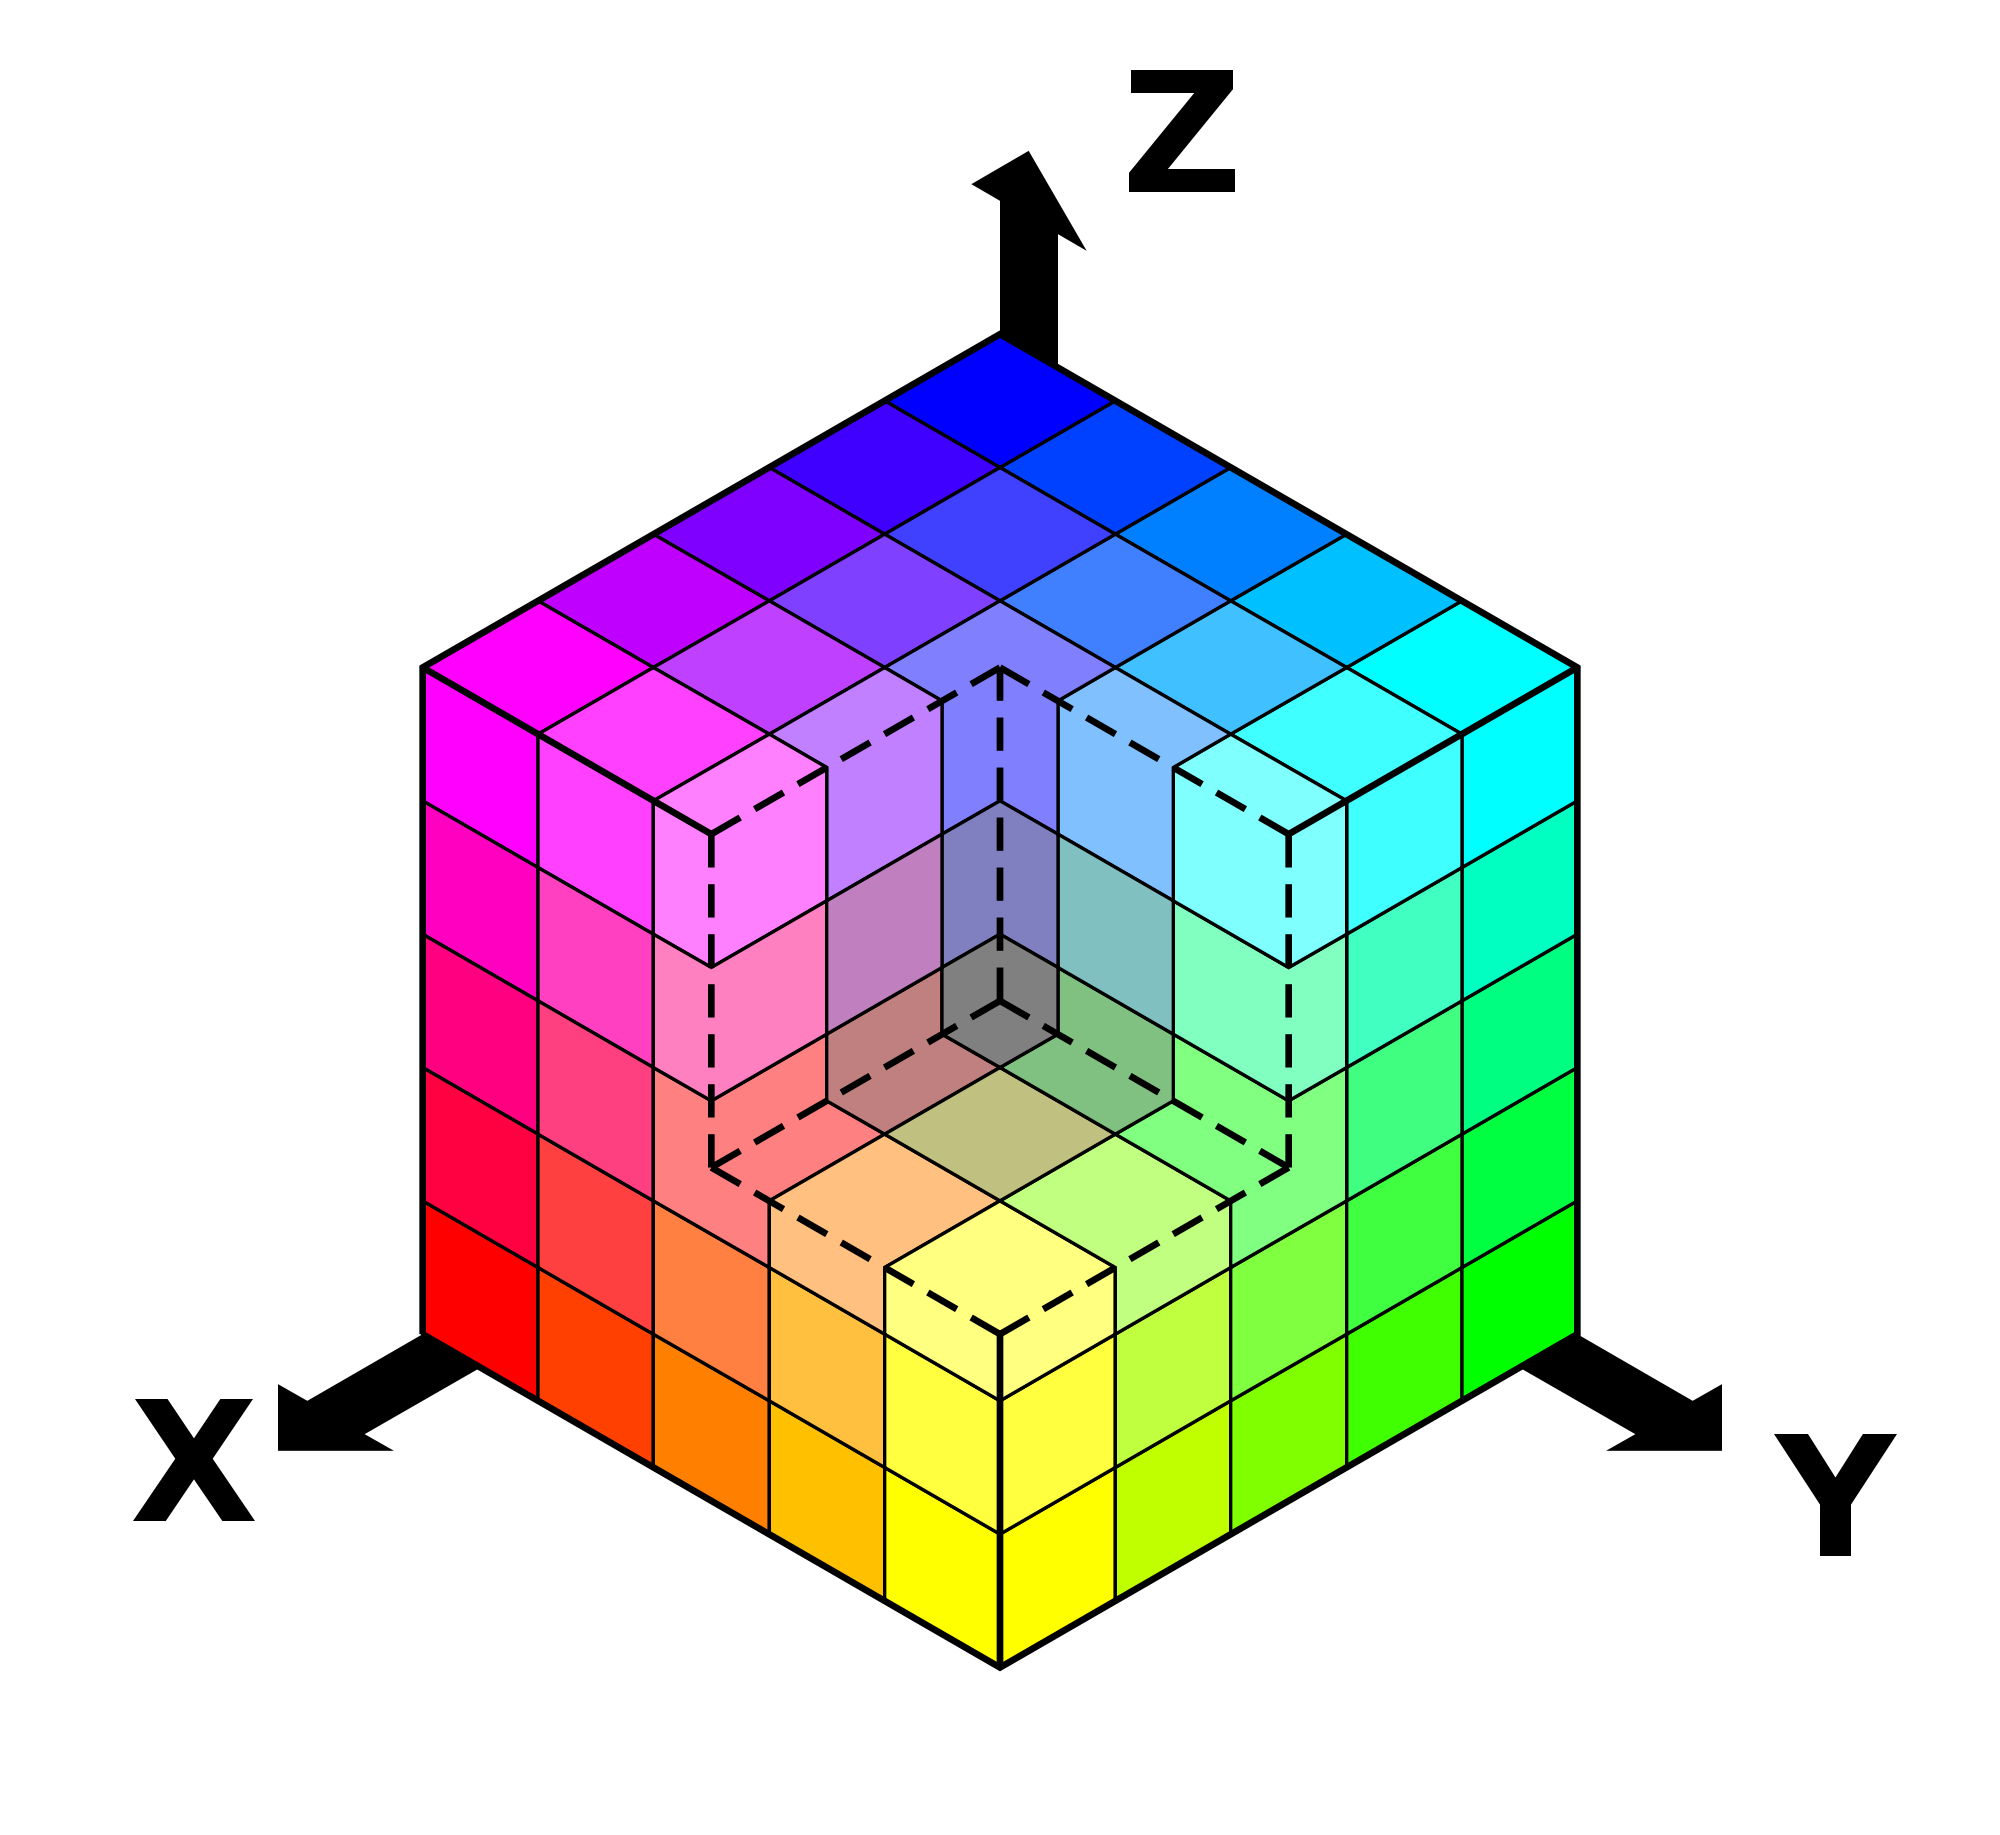
\includegraphics[width=.5\textwidth]{RGB_Model}
	\caption{Representation of the RGB Model \cite{_color}.}
	\label{fig:RGB_Model}
\end{figure}

\par In virtual environments, modeling is usually done using these primary colors in order to match the three types of cones in the human eye. The most frequently used model is the RGB model, representing red, green and blue colors. This model, seen in Figure \ref{fig:RGB_Model} allows any combination of colors to be created simply by combining a mixture of the three primary colors detectable by the human eye. 



\subsection{Depth Perception} \label{depth_perception} 


One of the most important functions of the human visual system is its ability to determine the distance to particular objects. This concept, known as depth perception, is extremely important in virtual realty. Since virtual displays do not always incorporate depth into a scene, VR designers must understand depth cues in order to fool the human senses and and create a virtual illusion of depth. The human mechanisms for determining depth can be divided into monoscopic and stereoscopic depth cues.

\par Monoscopic depth cues are received by just one eye and exist in two-dimensional images. From 
%\cite{vr tech and apps: pg. 99}
\cite{mihelj_apps}, Monoscopic depth cues include those listed below and several are depicted in Figure \ref{fig:depth}. 

\begin{figure}[h]
	\centering
	\includegraphics[width=.6\textwidth]{DepthPerceptionCues}
	\caption{Depth perception cues \cite{depth}\cite{texture}\cite{filippini}\cite{LinearPerspective}.}
	\label{fig:depth}
\end{figure}

\begin{enumerate}
	\item \textit{Occlusions:} Objects in the foreground obstruct those in the background.
	\item \textit{Shading:} Shading indicates the relative size of different objects and offers an estimate of their shape.
	\item \textit{Size:} Size allows comparisons between objects of different sizes, allowing us to gauge their relative distance.
	\item \textit{Linear Perspective:} Parallel lines appear to converge at a point as they recede into the distance. This can be used to determine the relative size, shape or position of an object by imagining or drawing these lines.
	\item \textit{Surface Texture:} Since the human eye cannot pick up sutle detail at great distances, objects further away have a less sharply defined texture than those that are closer.
	\item \textit{Accommodation:}  Accommodation is the dilation or contraction of the lens  in order to keep an object in focus as its distance from the eye varies. This process allows the brain to estimate the distance to an object based on the lens thickness.
	\item \textit{Parallax:} When the viewer is in motion, objects further away appear to move less in the field of view than objects that are closer to the view. 
	\item \textit{Movement of the view object:} When objects move further away from the viewer, they appear to grow smaller. When objects move closer to the viewer, they appear to become larger. This information allows the brain to estimate how long an approaching object has before it collides with the viewer.
\end{enumerate}





\par On the other hand, stereoscopic depth cues combine the information gathered from both eyes. Stereoscopic viewing is the primary way the visual system perceives depth. As objects become further than 30 meters away, many of the geometric benefits of stereopsis fade \cite{gobbetti}. This makes stereoscopic depth cues extremely effective for observing objects that are at closer distances. From \cite{mihelj_apps}, the stereoscopic depth cues are the following:


\begin{enumerate}
	\item \textit{Convergence:} The process where the eye turns inward toward an object in order to focus on that object, pictured in Figure \ref{fig:convergence}. This process allows the brain to judge the perceived depth of that object. 


	\item \textit{Stereopsis:} A process that allows depth to be estimated based on the difference between what the left and right eye perceive. 
\end{enumerate}


\begin{figure}[h]
	\centering
	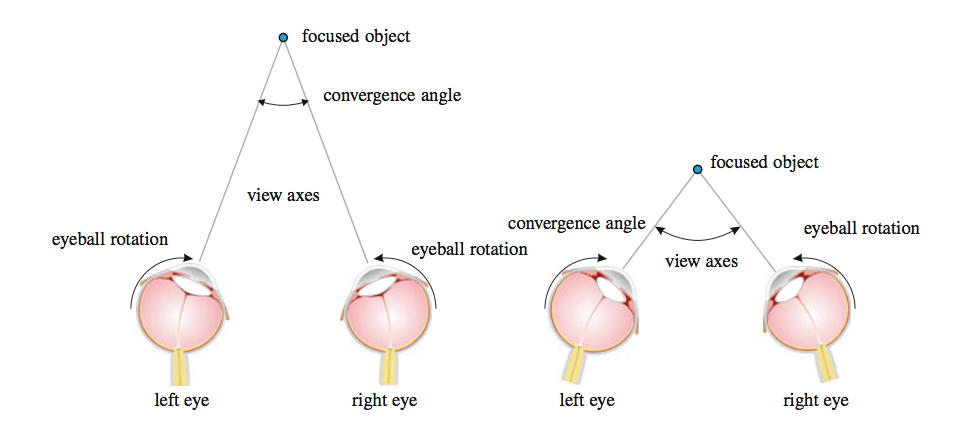
\includegraphics[width=.7\textwidth]{convergence}
	\caption{The Process of Convergence \cite{mihelj_apps}.}
	\label{fig:convergence}
\end{figure}

% cite haptics for VR and tele : pg 8
If there are conflicts between different depth cues, stereopsis takes precedence over all others \cite{mihelj_haptics}. A virtual environment can be designed using any of these cues to create a perceived feeling of depth. The more cues that are incorporated into a scene, the more realistic the illusion of depth becomes.


\subsection{Field Of View And Critical Fusion Frequency} \label{fov_criticalfusionfrequancy} 

Field-of-view, and critical fusion frequency also have an important role on the visual experience of immersive virtual scenes. The complete field of view for human eyes is around 180 degrees horizontally, and over 120 degrees vertically. Therefore, in order to create a successful optical illusion, the field of view should be 90 to 110 degrees \cite{gobbetti}. 
 
 
 \begin{figure}[h]
 	\centering
 	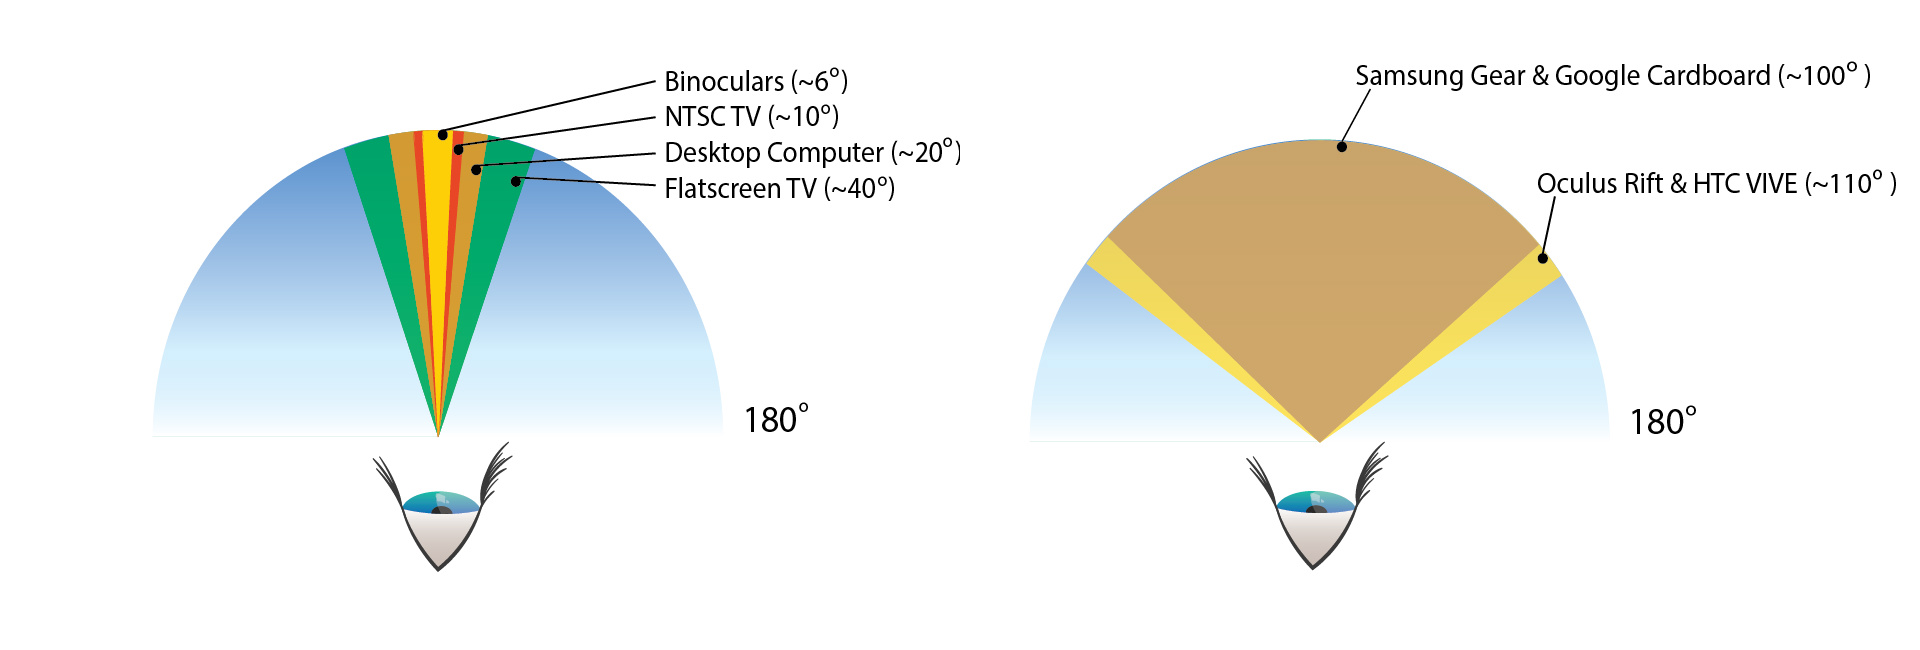
\includegraphics[width=.85\textwidth]{fov}
 	\caption{Field of view comparisons \cite{markiewicz_6_2015}.}
 	\label{fig:fov}	
 \end{figure}

 Different head mounted displays offer varying fields of views. As seen in Figure \ref{fig:fov}, the HTC Vive offers 110 degrees, an optimal field of view for VR applications. The critical fusion frequency is the rate that humans can distinguish between successive visual stimuli. For example, when the frequency is too small, object movement is choppy and no longer fluid. In computer graphics, a rate below 30-60 Hz results in this effect. 
 % do i remove this since it was already defined? or move it?
  

 \par  A narrow field of view and low frame rates in VR cause distraction and remind the user of their presence in a virtual setting. Visual displays, like the VIVE, require stereoscopic vision and must deliver stimuli of acceptable resolution, high-quality motion representations and satisfactory levels of brightness \cite{gobbetti}. Given the significance of the visual system, visual displays have become the most important piece of VR hardware. However, head mounted displays are not always enough. Virtual environments should not only engage a user's visual and auditory senses, but also offer user interaction mechanisms. Haptic hardware is able to create interactive connections between the user and their environment, an aspect absolutely critical in achieving an immersive application.
 
 \begin{figure}[h]
 	\centering
 	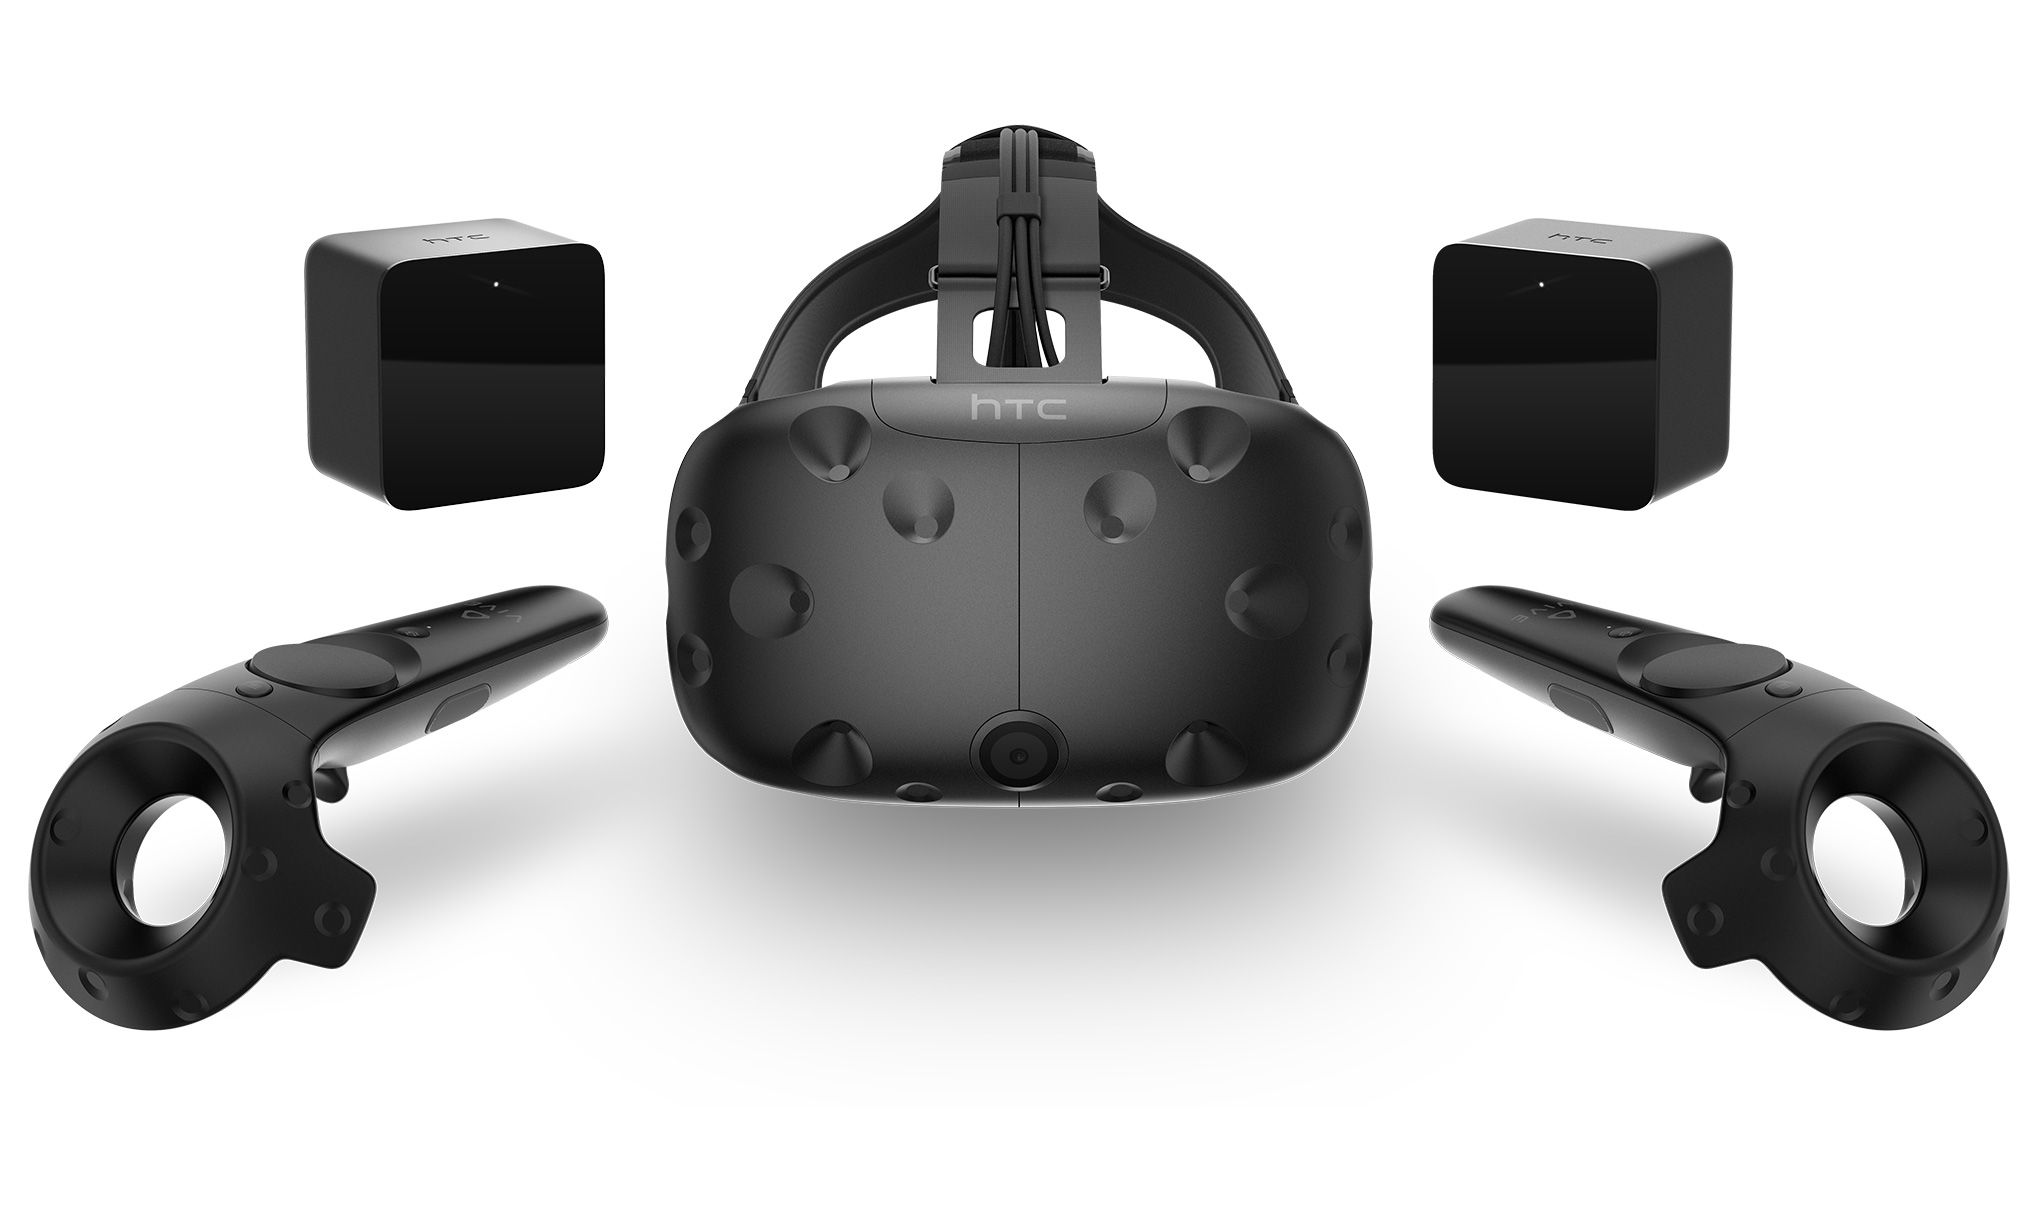
\includegraphics[width=.6\textwidth]{htc_vive}
 	\caption{HTC Vive with hardware - including haptic controllers \cite{walton_psvr_2016}.}
 	\label{fig:vive}
 \end{figure}


 
 
 %%%%%%%%%%%%%%%%%%%	
 %				   %	
 %      TOUCH      %
 %				   %
 %%%%%%%%%%%%%%%%%%%
 

\section{Human Haptic System} \label{touch}

% + definition of haptics
% + haptic perception
% + haptic applications?
% + haptic representation in VR
% + haptic rendering in VR


% intro: definition of haptics

The word \textit{haptic} comes from the Greek verb \textit{hapto}, meaning \textit{to touch}. %cite hapticsfor VR pg 35
Haptic refers to the exploration and process of identifying objects through touch \cite{mihelj_haptics}. %cite haptics for VR pg.10
An effective VR system utilizes haptic devices to enable a user to interact with objects in a virtual environment through gestures. Figure \ref{fig:vive} shows the HTC Vive, an example of a commercially popular head tracking system that is also equipped with haptic controllers. A haptic device mimics tasks that would normally be performed in the real world, such as gathering information about an object and its properties. A haptic interface is a device that measures a position or contact force and displays that contact force or position to the user. To put it even more simply, a haptic interface receives motor commands from the user and displays haptic images back to the user \cite{mihelj_haptics}. The human hand allows a user to push, grasp, squeeze or hit objects. When transfered into a virtual space, being able to touch, feel and manipulate objects results in a level of immersion that is not possible without a haptic system. Haptic hardware in VR allows the user to perceive information about the virtual world, and the rules that govern it. Many new games use haptic hardware that allows the user to interact and manipulate objects in the virtual world. A game called Job Simulator, illustrated in Figure \ref{fig:job_simulator}, implements these strategies to allow the user to interact with objects as part of the storyline. The inability to have this level of interaction within an environment makes it impossible for a user to truly perceive a virtual world as real. 


\begin{figure}[h]
	\centering
	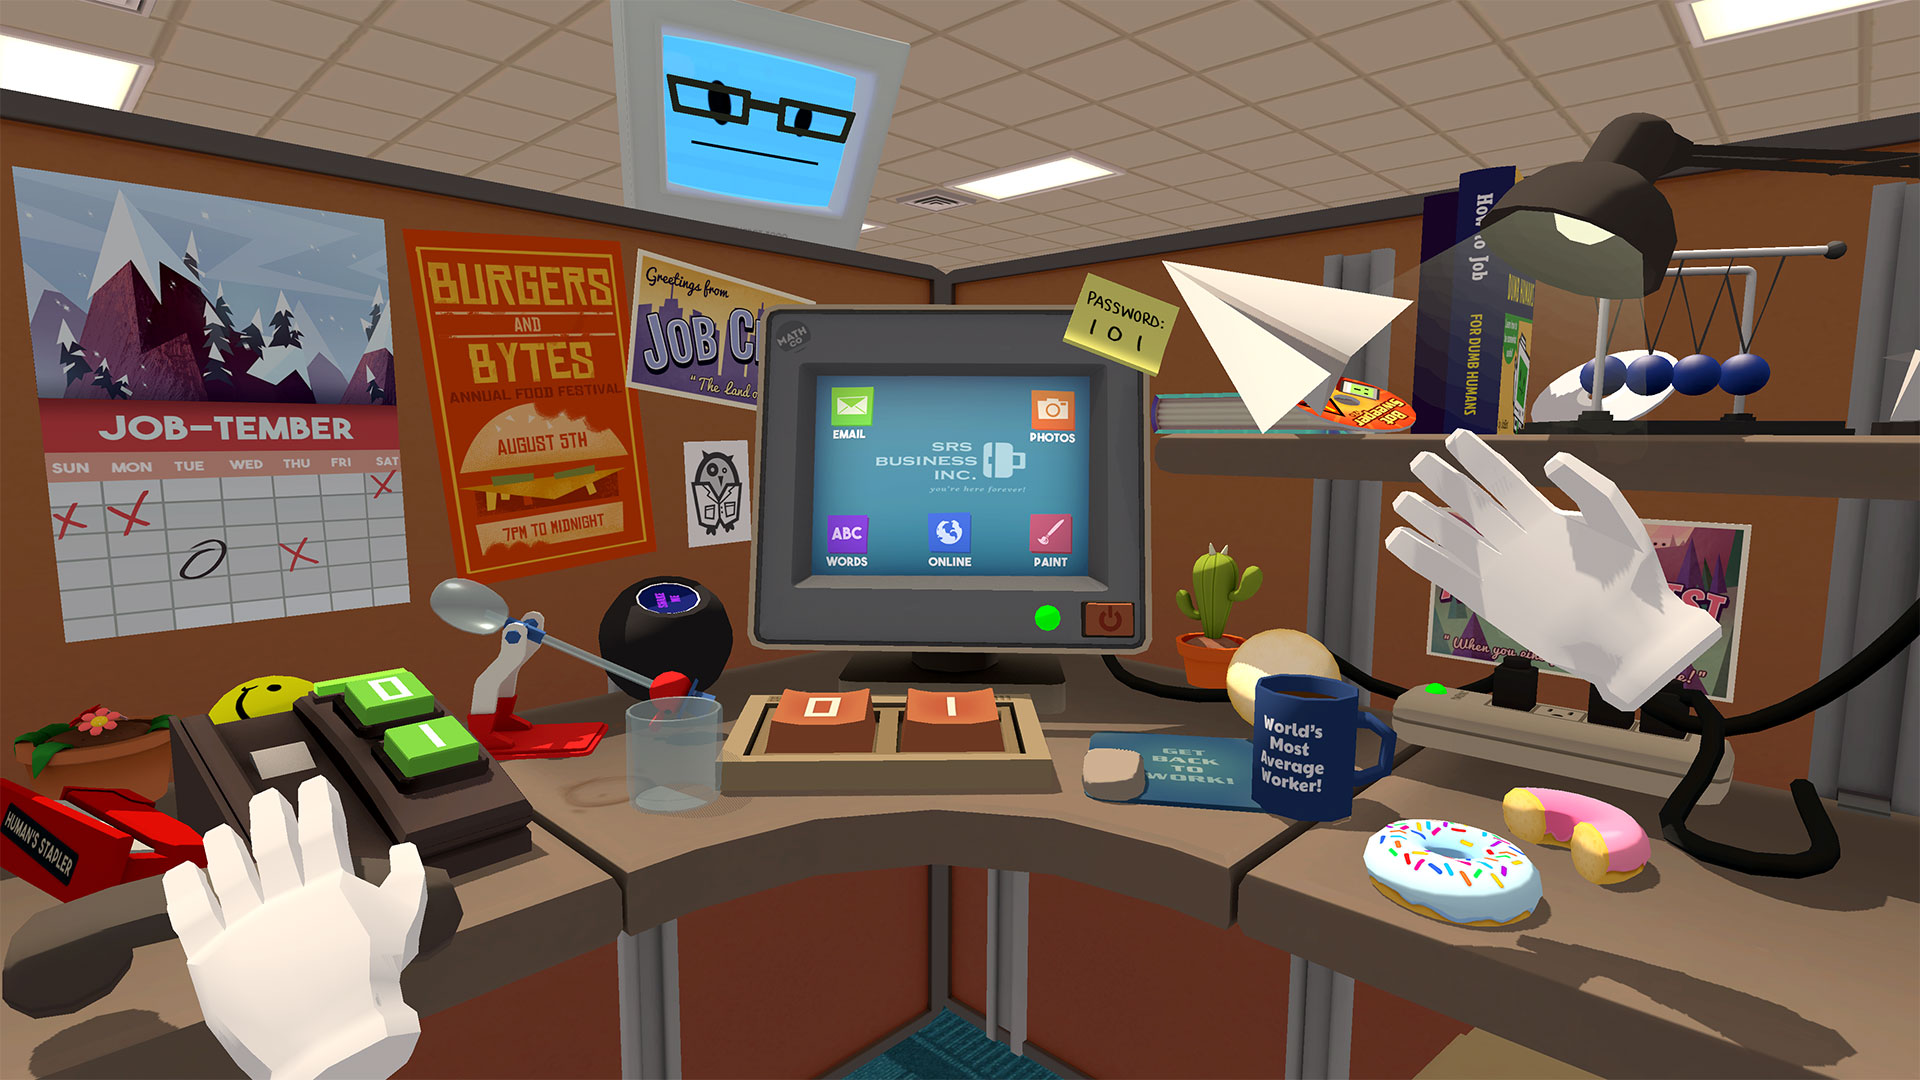
\includegraphics[width=.7\textwidth]{job_simulator}
	\caption{Job Simulator: An interactive game that uses haptic hardware and object manipulation as it's primary tool for creating an immersive experience \cite{jobSim}.}
	
	\label{fig:job_simulator}
\end{figure}

%  haptic perception (basics)
 \par Haptic perception is different from vision and sound because it provides the ability to sense and also act upon an environment. Through touch, different types of information can be gathered when manipulating objects in the environment. The human haptic system is divided into three subsystems made up of sensory capabilities, motor capabilities and cognitive capabilities. Sensory capabilities use kinesthetic and tactile senses to derive information about the environment through touch. In VR, sensory capabilities can be used to give the user cues and insight on the virtual world and its rules. Motor capabilities use the musculoskeletal system to gain information about and manipulate objects through interaction. Cognitive capabilities use the central nervous system to analyze information gathered from an environment and plan motor functions based on the objectives of the tasks. When designing haptic interfaces, understanding the haptic system is imperative.



%%%%%%%% this seems repetitive %%%%%%%%
%The information gathered can be characterized as either tactile or proprioceptive \cite{gobbetti}. Tactile information is gathered from an initial touch of an object. This provides knowledge of the shape and the texture of the object. Applying extended force to an object provides proprioceptive information of the object's weight, forces acting upon the object and surface compliance \cite{gobbetti}. Combining tactile and proprioceptive cues allows the user to feel present and engaged within a virtual setting.
%%%%%%%% This also seems reptitive %%%%%%%%
%A haptic experience is based on tactile and kinesthetic senses. Tactile senses provide information based on the stimuli on the surface of the body. Kinesthetic senses give information about the pose and movement of the body.



\subsection{Sensory System} \label{tactile_kinesthetic}

 % explain active verse inactive movement...?
 \par Sensory information can be broken further into subclasses consisting of tactile and kinesthetic information. Tactile sensors transmit information to the brain about an object when initial contact is made. This information is gathered by low-threshhold mechanoreceptors  in the skin such as a fingertip \cite{mihelj_haptics}. When the hand is stationary and comes into contact with an object, tactile sensors are the ones to transmit information concerning that object. The type of information gathered by tactile sensors can range from the fine texture, size, softness, slipperiness and temperature of an object. On the other hand, kinesthetic information conveys the position, movement and forces acting on a limb \cite{mihelj_haptics}. When an arm or other limb is active in free space, this kinesthetic information gives insight regarding the natural shape, compliance and stiffness of surrounding objects. During any active task, sensory information is simultaneously gathered from both types of sensors, giving the brain constant feedback.
 
 \subsubsection{Kinesthetic Perception} \label{tactile_kinesthetic}
 
 The Kinesthetic system is primarily used to acquire information about the forces generated by certain muscles, and the resulting movement of limbs. However, kinesthetics also refers to the perception of force, an aspect extremely relevant in the topic of haptic interaction systems within virtual reality. Mechanoreceptors provide information to the central nervous system about static muscle length, muscle contraction velocity, and forces generated by muscles \cite{mihelj_haptics}. Other sensory information regarding the change of limb position are acquired from receptors in the joints and skin. The receptors in the skin play an important role in tactile exploration and interpreting the position and movement of the arms. This subsection gives an overview of the kinesthetic receptors, specifically mechanoreceptors, which are responsible for the perception of movement, force, and the position of limbs.
 
 \par  Mechanoreceptors are found in muscle spindles and are classified as primary and secondary receptors. Seen in Figure \ref{fig:receptors}, muscle spindles, found in muscles, are .5-10 mm in length and made up of bundles of muscle fibers \cite{mihelj_haptics}. Muscle fibers are attached at both ends to muscle or tendon fibers and are responsible for generating muscle force. These spindles identify changes of tension and length within muscle fibers. The primary role of muscle spindles is to act as an automatic safety device for the muscles. When the muscle is overly stretched, the spindles respond by stimulating a muscle contraction in order to prevent the muscle from extending or stretching too far. These automatic muscle contractions, or reflexes, are important for controlling movement and balance.
 
 
 \begin{figure}[h]
 	\centering
 	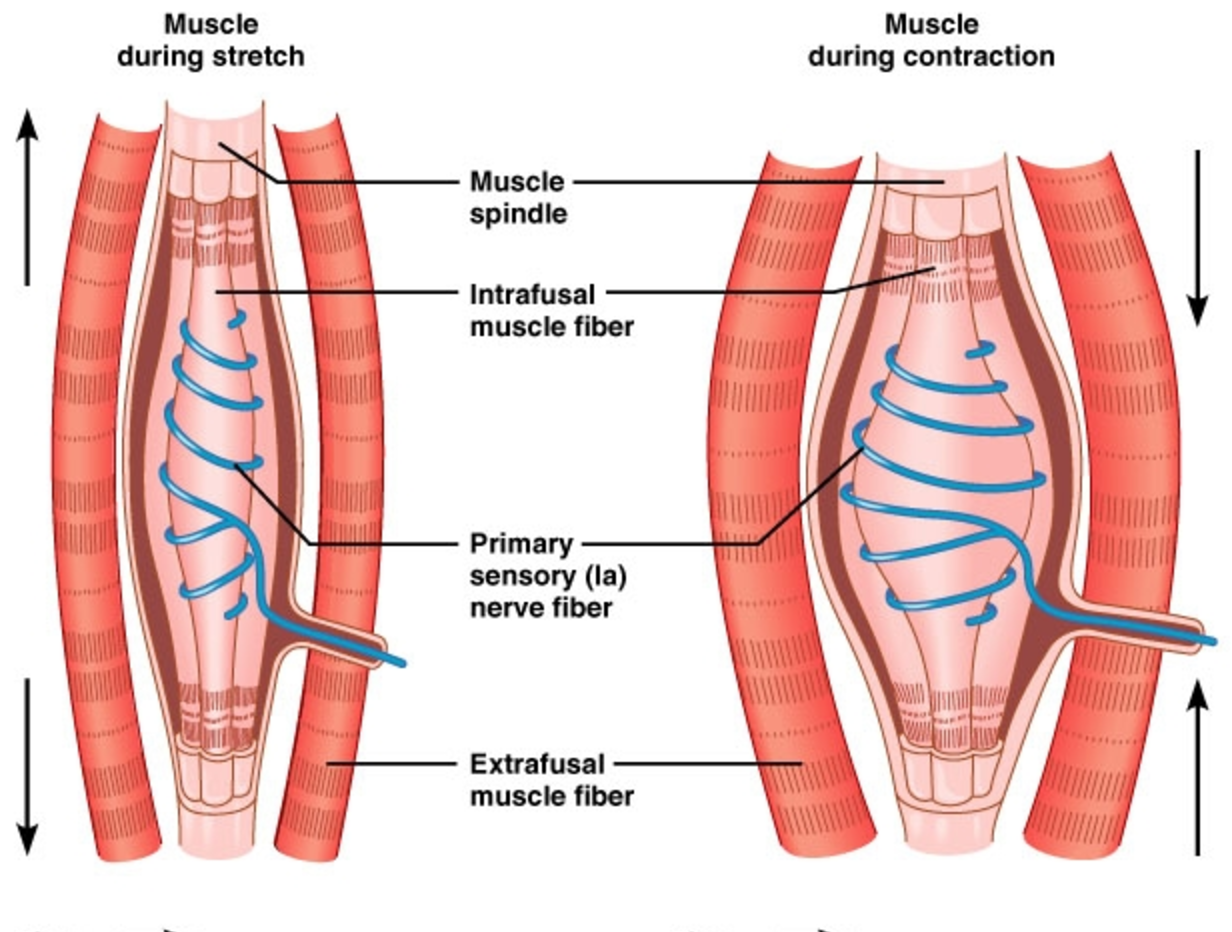
\includegraphics[width=.6\textwidth]{receptors}
 	\caption{Kinesthetic Receptors \cite{proprioception}.}
 	\label{fig:receptors}
 \end{figure}


 % Both primary and secondary spindle receptors respond to velocity, direction, movement, length and position of the lib. 
 

\par Each mechanoreceptor, primary and secondary, react to a change in muscle length and act accordingly. The primary spindle receptors dynamically respond to changes in muscle length by dealing with the velocity and acceleration aspects of movement. The job of the primary receptors is to modify the sensitivity of muscle spindles based on the muscle's length, contraction history, and current velocity of muscle contractions \cite{mihelj_haptics}. Primary receptors actively influence the velocity, direction and movement of a limb. In contrast, the secondary receptor's job is to output a constant static measurement of muscle length and position of the limb. Normally, an area with a high density of mechanoreceptors  means a highly functional tactile system. However, in a kinesthetic system, a higher density of receptors does not always mean better kinesthetic capabilities \cite{mihelj_haptics}. Instead, the size of the muscle, not the functionality, dictates the number of muscle spindles present. 


 
\begin{figure}[h]
	\centering
	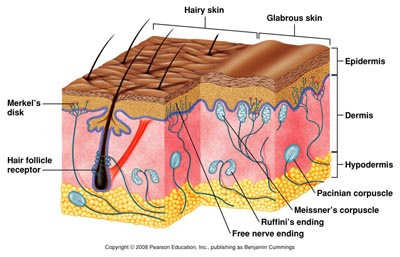
\includegraphics[width=.75\textwidth]{SkinReceptors}
	\caption{Ruffini Endings and Pacinian Corpuscles \cite{somatosensory}}
	%\cite: http://www.d.umn.edu/~jfitzake/Lectures/DMED/Somatosensation/Somatosensation/Receptors.html
	\label{fig:SkinReceptors}
\end{figure}


\par In addition to spindle receptors, there are other types of mechanoreceptors used within the human haptic system, displayed in Figure \ref{fig:SkinReceptors}.
Located where the tendon attaches to the bundle of muscle fibers, the Golgi tendon organ provides information about force exerted by muscles \cite{mihelj_haptics}. The Golgi tendon organ essentially serves as a safety mechanism by reducing muscle tension when the muscle is under an excessive load.  Ruffini endings and the Pacinian corpuscles are other mechanoreceptors found in the joints. The Ruffini endings sense angle and angular velocity of the joint movements. The Pacinian corpuscles are used to estimate joint acceleration and have a natural sensitivity that responds to both vibration and pressure \cite{mihelj_haptics}.


 \subsubsection{Tactile Perception}
 
 


 While the kinesthetic system works to acquire information regarding force and the movement of limbs, the tactile system defines and interprets sensations acquired through touch. The various and complex sensations generated during object interaction are made up of a few specific components. Roughness, lateral skin stretch, relative tangential movement and vibrations make up the sensations we receive when interacting with these objects \cite{mihelj_haptics}. The mechanoreceptors in the skin define the texture, shape, compliance and temperature that are all perceived through touch. Specifically, the Meissner's corpuscles, Pacinian corpuscles, Markel's disks and Ruffini corpuscles are the sensory organs in the skin that define a sensory experience. These sensory organs and their properties are displayed in Figure \ref{fig:Mechanoreceptors}
 
 
  \begin{figure}[h]
 	\centering
 	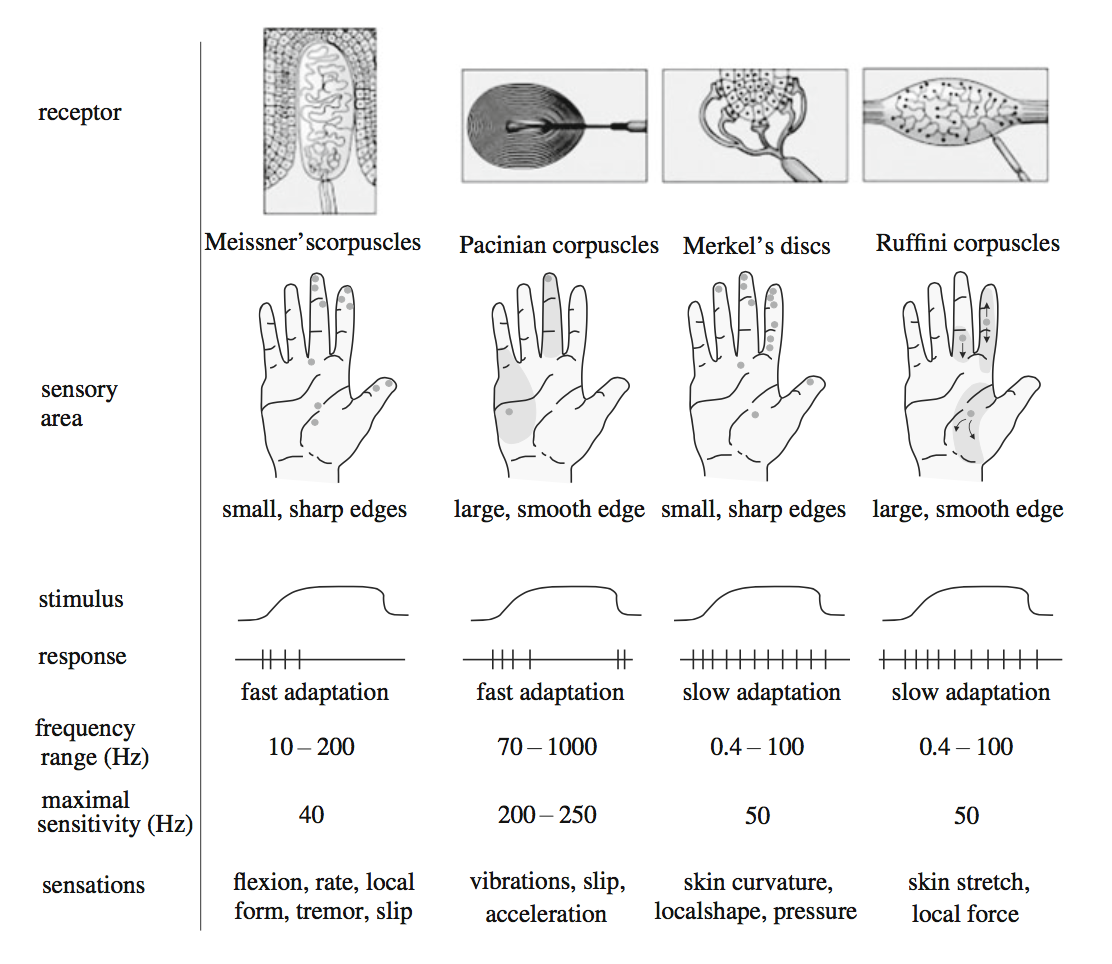
\includegraphics[width=.6\textwidth]{Mechanoreceptors}
 	\caption{Properties of Mechanoreceptors \cite{mihelj_haptics}.}
 	\label{fig:Mechanoreceptors}
 \end{figure}

 \par These four types of mechanoreceptors differ in size, receptive fields, rate of adaptation, location in the skin and physiological properties. Spatial resolution depends on where the receptors are located in the skin. Certain receptors have large receptive fields, which means they have a low spatial resolution. Others have small receptive fields, meaning they have a good spacial resolution. Each receptor also has a different rate of adaptation. When a receptor has fast adaptation, it detects short pules of sensory information. An example of fast adaptation is the initial contact with an object or the detection of a vibration. A slow speed of adaptation means the receptor detects a constant stimulus, like a constant pressure. Figure \ref{fig:Mechanoreceptors} displays the rate of adaptation of receptors in the skin. 
   


 \par Like color perception, the quality of a sensory experience is determined by a combination of responses from different receptors. Receptors are able to achieve a wide detection range for detecting vibrations and frequencies ranging from 0.4 to 1000Hz \cite{mihelj_haptics}. Frequencies over 500Hz are no longer felt as vibrations, but as having textural qualities. Given the properties of a tactile system, specifically the perception area, duration and frequencies are important for modeling interaction systems in virtual environments.


 
\subsection{Motor and Cognitive Systems} \label{motor_cognitive}
 
 
 \begin{figure}[h]
 	\centering
 	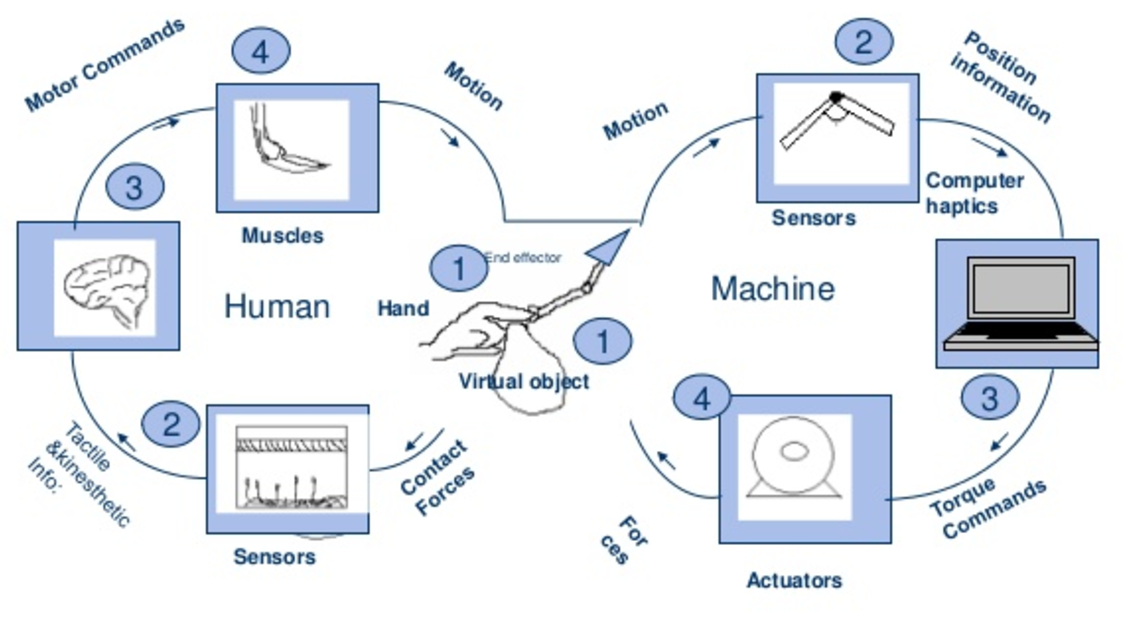
\includegraphics[width=.8\textwidth]{haptic_interaction}
 	\caption{Human-Machine Haptic Interaction \cite{ganesan}.}
 	\label{fig:haptic_loop}
 \end{figure}
 
 
  \par In addition to sensory capabilities, the motor system and the cognitive system make up the human haptic system. The motor system allows for active exploration of an environment and manipulation of objects within it.  The cognitive system associates action with perception \cite{mihelj_haptics}.  When designing a haptic experience in VR, understanding how these different haptic subsystems function and work enables a designer to build an interactive and realistic virtual environment. Figure \ref{fig:haptic_loop} displays how the haptic subsystems work together with a haptic hardware device to control the position of the hand and exert forces to simulate contact with a virtual object. The sensory, motor and cognitive systems all work together to construct a haptic experience. Both tactile and kinesthetic sensory information compose contact perception, while motor commands allow movement and navigation through an environment based on the cognitive objectives \cite{mihelj_haptics}. The more haptic subsystems used to define a virtual experience, the more a user feels engaged and immersed within that experience. 
 
 



 %%%%%%%%%%%%%%%%%%%	
 %				   %	
 %      SOUND      %
 %				   %
 %%%%%%%%%%%%%%%%%%%

\section{Aural System} \label{sound}

While vision is primarily used for virtual perception and haptic controllers provide interaction systems, the use of sound is invaluable. Visual systems provide spatial information about an environment that exist in both space and time. In contrast, aural systems provide temporal information in a virtual space that exist in time and not space. The timing of sound presentation is therefore even more critical than the timing of image presentation in VR \cite{mihelj_haptics}. In addition, since sound is perceived the same no matter what direction a user is facing, sound is not limited by the orientation of the head. When realistically implemented, sound increases the feeling of mental immersion and provides informative cues about a virtual environment. Hearing and sound perception allow for verbal communication. Verbal communication increases situational awareness, cues visual attention and presents complex information that vision cannot always provide us. Audio perception requires the ability to synthesize sound and to locate and pinpoint auditory stimuli within a 3D space. The most efficient hearing frequency in humans occurs between 1000 and 4000 Hz \cite{gobbetti}.%[quote page 8] 
Hearing is classified as a remote sense because it is used to detect the position of objects relative to a user. 


\par Given that VR exists in three-dimensional space, three-dimensional sound must be implemented. A concept called \textit{sound localization} represents a phenomenon that allows users to identify the distance and direction of a detected sound source \cite{mihelj_haptics}.  Within a virtual environment, auditory stimuli can be generated using location-dependent filters to enhance a users virtual presence. In such environments, Stereo, or auditory, clues can be given for the users to evaluate. These stereo clues can exist for the users to make assumptions on elevational changes or to determine directivity \cite{gobbetti}. Sounds can also be generated to approximate distance. Since sound decays the further away it is, the amplitude of a sound can be used as a distance cue for a user. Creating an illusion that sound originates from specific points in virtual environment creates a sense of realism for the user. 

\begin{figure}[h]
	\centering
	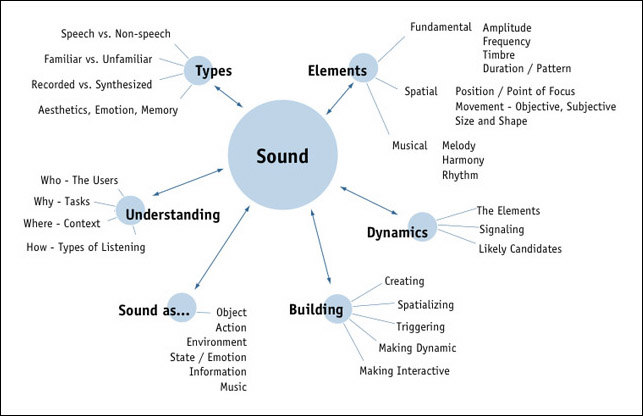
\includegraphics[width=.7\textwidth]{photo8_sound}
	\caption{The Complex Nature of Auditory Processing \cite{sound}}
	\label{fig:soundPerception}
\end{figure}

\par The challenge for auditory implementation in virtual environments stems from the complexity of auditory perception, illustrated in Figure \ref{fig:soundPerception}. Different types of sounds attract different types of attention. Ambient sounds give clues about the size and nature of an environment. The desired mood of an virtual environment is constructed through different ambient sounds. Individual objects can have sounds associated with them to give an understanding of each object and to demonstrate different possible actions that can accomplished with each object. Auditory processing is absolutely crucial but often overlooked in virtual settings due to the complexity of implementation. 

% speak about acoustic rendering? page 16 - haptics


\section{Design Guidelines} \label{Guidelines}




\section{Conclusion} \label{Guidelines}











